\documentclass[a4paper,twoside]{article}
\usepackage[T1]{fontenc}
\usepackage[utf8]{inputenc}
\usepackage{epsfig}
\usepackage{subcaption}
\usepackage{calc}
\usepackage{amssymb}
\usepackage{amstext}
\usepackage{amsmath}
\usepackage{amsthm}
\usepackage{multicol}
\usepackage{pslatex}
\usepackage{apalike}
\usepackage{algorithm2e}
\usepackage[bottom]{footmisc}
\usepackage{booktabs}
\usepackage{url}
\usepackage[hidelinks,pdfauthor={},pdftitle={Contextual Ontology Extraction and Inspection of Temporal Narrative Networks},pdfcreator={LaTeX},pdfsubject={Anonymous position paper}]{hyperref}
\usepackage{SCITEPRESS}
\newcommand{\Temperature}{0.7}
\newcommand{\TopP}{0.8}
\newcommand{\TopK}{20}
\newcommand{\Seed}{1988649846}
\newcommand{\OutputTokens}{2,048}
\newcommand{\ContextTokens}{12,288}
\newcommand{\StorySentences}{14}
\newcommand{\FableWords}{133}
\newcommand{\AliceWords}{112}
\newcommand{\HolmesWords}{159}
\newcommand{\CompactCalls}{12}
\newcommand{\ProseCalls}{9}
\newcommand{\ProseParsed}{7}
\newcommand{\IntervalsKept}{79}
\newcommand{\IntervalsEligible}{79}
\newcommand{\OrchardLocationRecall}{0.750}
\newcommand{\MainCalls}{21}
\newcommand{\MainAllocation}{454.82}
\newcommand{\CompactAllocation}{249.45}
\newcommand{\ProseAllocation}{205.37}
\newcommand{\CompactRequest}{104.72}
\newcommand{\ProseRequest}{57.24}
\newcommand{\FableAFone}{0.625}
\newcommand{\FableACoverage}{6 of 8}
\newcommand{\FableBFone}{0.308}
\newcommand{\FableBCoverage}{4 of 8}
\newcommand{\AliceAFone}{0.000}
\newcommand{\AliceACoverage}{1 of 4}
\newcommand{\AliceBFone}{0.000}
\newcommand{\AliceBCoverage}{3 of 4}
\newcommand{\FableQuestion}{Which physical running/waking, capture, binding, rope-gnawing and release relationships involve the Lion, Mouse, hunters and ropes? Exclude dialogue, intentions, laughter and the moral.}
\newcommand{\HarborQuestion}{Which directly narrated location relationships have an explicitly stated interval overlapping day 2 up to but not including day 4? Return all of them with their full evidence-stated intervals, not clipped to the question window. Exclude undated locations and beliefs.}
\newcommand{\OrchardQuestion}{Who owns or carries what? Return all and only directly narrated ownership and carrying relationships, retaining every stated interval.}
\newcommand{\OrchardBeliefQuestion}{Who explicitly believes what, and what reality is separately narrated about those same objects? Return each underlying believed relationship with its attribution and each matching narrated reality without attribution. Omit unrelated facts.}
\newcommand{\AliceActionQuestion}{Which sitting/location, reading/inspection and running relationships involve Alice, her sister, the book, bank and Rabbit? Exclude thoughts, feelings, appearance and book-content properties.}
\newcommand{\AliceClaimQuestion}{What does the passage say about the book's absent content and Alice's thoughts about the usefulness of such books and making a daisy-chain? Exclude physical actions, locations, appearance and the Rabbit; preserve questions and consideration without treating them as decisions.}

% Conference-native artwork: figures are NOT scaled-down general-paper plates.
\newcommand{\FableFigure}{
\begin{figure*}[!t]
\centering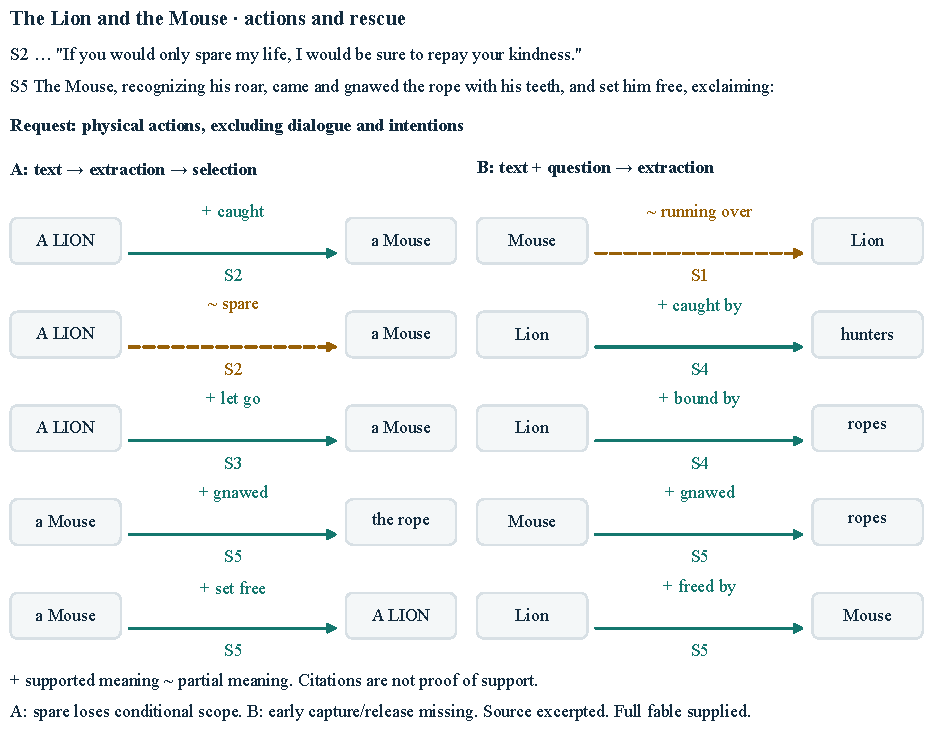
\includegraphics[width=\textwidth]{figures/fable.pdf}
\caption{Fable action records from fixed selection (A) and contextual extraction (B). + marks supported meaning; $\sim$ marks partial meaning.}
\label{fig:fable}
\end{figure*}}
\newcommand{\OrchardFigure}{
\begin{figure*}[!t]
\centering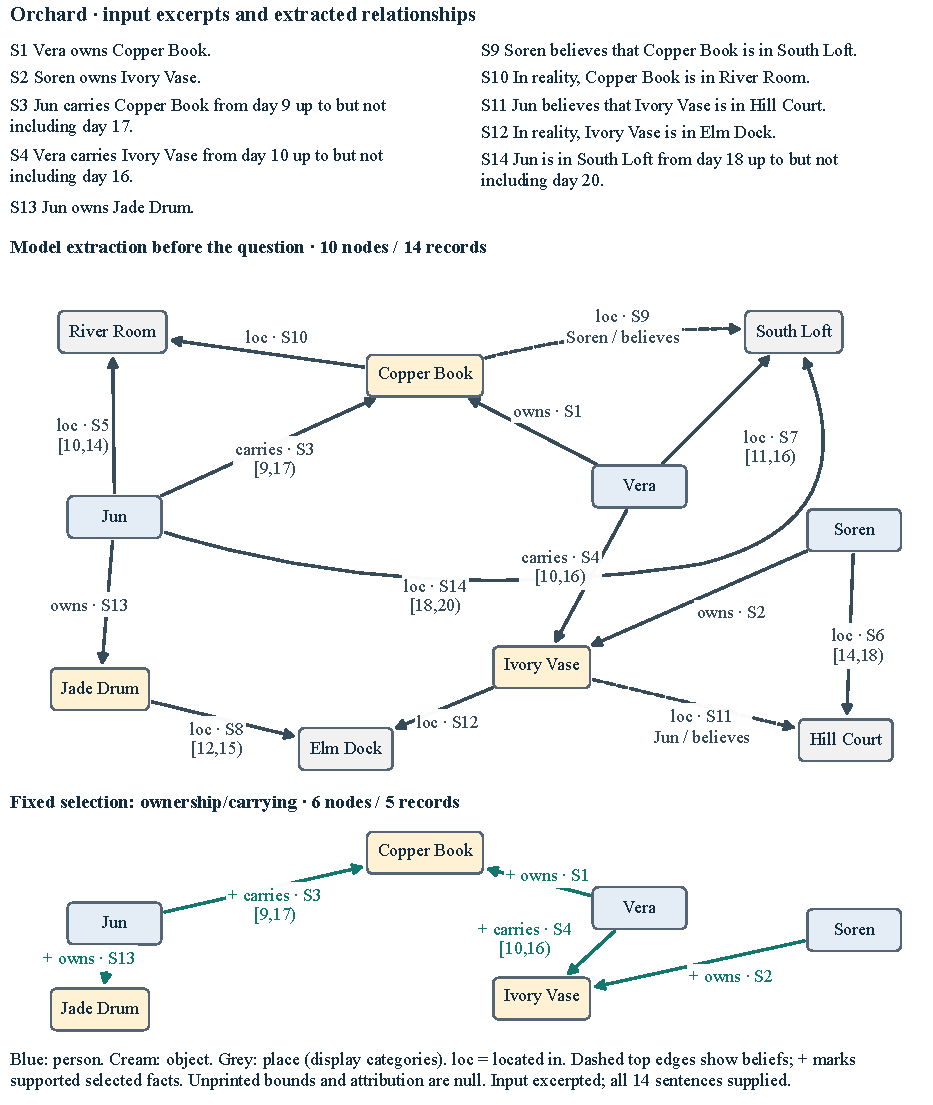
\includegraphics[width=\textwidth]{figures/orchard_network.pdf}
\caption{Orchard input excerpts, model extraction (top network) and fixed ownership/carrying selection (bottom). Believer names qualify edges; they do not add relationships.}
\label{fig:orchard}
\end{figure*}}
\newcommand{\AliceFigure}{
\begin{figure*}[!t]
\centering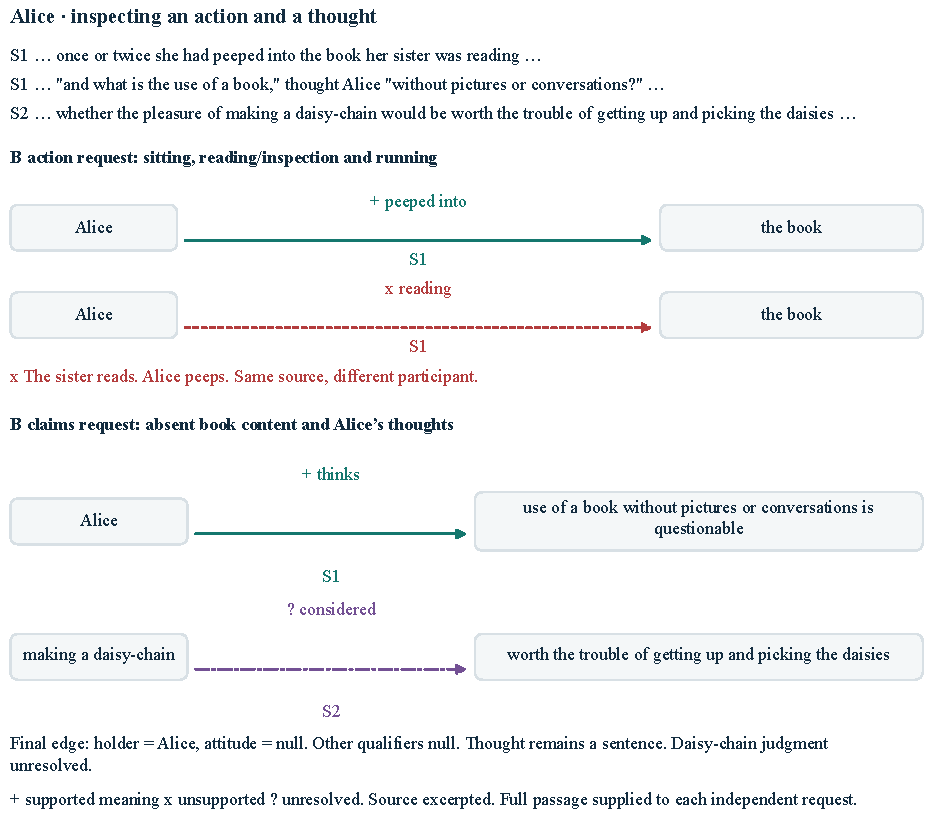
\includegraphics[width=\textwidth]{figures/alice.pdf}
\caption{Alice's contextual action and thought records. + marks supported meaning, x a wrong participant, and ? an unresolved interpretation.}
\label{fig:alice}
\end{figure*}}

\begin{document}
\title{Contextual Ontology Extraction and Inspection of Temporal Narrative Networks}
\author{}
\keywords{Natural Language Processing, Knowledge Representation and Reasoning, Large Language Models, Visualization.}
\abstract{We present a narrative extraction workflow connecting readers' questions, generated relationships, temporal and attribution details, and visual inspection of evidence and errors. We compare extraction before seeing a question followed by fixed selection with independent contextual extraction on three synthetic stories and three short published passages. Assessment separates strict agreement with reference answers from preserved meaning, relevance and unresolved interpretation. All \CompactCalls\ story responses were parseable. Fixed selection matched every possession and dated location target without extras, whereas contextual answers retained irrelevant facts. On fable actions, strict F1 was \FableAFone\ for selection and \FableBFone\ for contextual extraction. Query-guided extraction of statements and thoughts from an excerpt of Alice’s Adventures in Wonderland preserved \AliceBCoverage\ semantic targets despite zero strict F1. Prose parsing succeeded in \ProseParsed\ of \ProseCalls\ calls. The workflow makes these mixed results  easy to inspect, including useful thought representations, incorrect participants and lost conditional scope. These small development comparisons identify concrete extraction and selection problems for further research. }
\onecolumn\maketitle\normalsize\setcounter{footnote}{0}\vfill

\section{\uppercase{Introduction}}
\noindent Stories describe people, places and objects whose relationships change over time. Readers may ask who carries an object, where it is, or what a character believes about it. A comprehensive graph can obscure an answer; extracting only for a question can omit needed facts. Our workflow explores narrative ontologies: local vocabularies and records of story entities and relationships. A temporal ontology also represents when relationships hold; here, intervals qualify the records. The network displays entities as nodes and relationships as edges. Source links distinguish beliefs from narration. This is a compact representation, not a complete formal theory of the story.

We compare two ways to produce a network for a reader's question. \emph{Pre-extract/select} (A) first extracts relationships without seeing the question, then selects existing records using fixed filters. \emph{Contextual extraction} (B) extracts relationships directly from the same text with the question supplied. Both use records with entity names, evidence citations, time intervals and attribution. Our contributions are:

\begin{enumerate}
\item An implemented workflow connecting narrative questions, temporal networks and source evidence. Linked views let readers inspect relationships and trace their meaning to the text (Section~3 and Figures~\ref{fig:orchard}-\ref{fig:alice}).
\item An empirical comparison of extraction before and after the question is supplied. Results on synthetic stories and published prose help distinguish problems in extracting relationships from problems in selecting relevant ones (Section~5).
\item An assessment combining agreement with reference answers, preservation of meaning, relevance and unresolved interpretation. Tables~\ref{tab:compact} and~\ref{tab:prose} and the annotated networks show useful partial results alongside errors.
\end{enumerate}

This is an exploratory implementation and comparison, not a new extraction algorithm. Section~2 relates it to existing work; Section~3 explains the records and two approaches; Sections~4--5 describe evaluation and results; Sections~6--7 discuss limitations and next steps.

\OrchardFigure
\section{\uppercase{Related Work}}
\noindent \emph{Extraction and representation.} TextRunner is an early example of extraction without a predefined relation vocabulary \cite{banko2007}, not our experimental baseline. ReVerb constrains relation phrases \cite{fader2011}; OLLIE also retains attribution and conditional context \cite{mausam2012}. SPIRES uses recursive LLM prompts to fill a supplied schema and link entities to vocabularies \cite{caufield2024}. We compare question timing with one LLM, not these systems' extraction accuracy.

Temporal ontologies provide a foundation for describing change. OWL-Time represents instants, intervals, durations and ordering \cite{time2017}. GRaSP connects statements, textual mentions, sources and attitudes, with an interface linking events to their evidence \cite{fokkens2017}. These foundations inform our compact representation of when relationships hold and who expresses a belief.

ATOM builds and updates temporal knowledge graphs from small facts, distinguishing observation time from validity time \cite{lairgi2026}. We instead compare question-guided extraction with fixed selection; we do not test graph updating or establish an advantage over ATOM.

\emph{Comparison and inspection.} RelVis combines extraction comparison, visual inspection and error annotation \cite{schneider2017}. It also distinguishes valid relationships missing from reference annotations from extraction errors. CaRB improves reference annotations and scoring through partial coverage and checks on the alignment of relationships and their participants \cite{bhardwaj2019}. Using our own strict matcher, we report agreement separately from judgments about preserved meaning, missing details and unresolved readings.

Our visualization draws on established filtering, linked selection and coordinated views \cite{heer2012}. We use these views to compare answers to the same story question and to check each relationship against its source, including its time interval and whose belief it expresses.



\section{\uppercase{Representation and Methods}}


\subsection{Evidence and Qualified Records}
\noindent Each request receives the complete selected story or contiguous excerpt with unchanged wording and numbered evidence spans. Each extracted relationship is represented by a qualified record:
\begin{equation}
\label{eq:qualified-record}
f = \langle s, r, o, E, t_0, t_1, h, a \rangle .
\end{equation}
The subject $s$, relation $r$ and object $o$ define an edge; $E$ cites its evidence and $t_0,t_1$ give its temporal bounds. Attribution identifies whose statement or belief is recorded: holder $h$ names the person; attitude $a$ specifies, for example, \texttt{believes} or \texttt{promises}. The model supplies every value; the runtime never fills missing meaning from reference answers.

The following illustration is authored to explain the format and is not a model result:
\begin{small}\begin{verbatim}
{"subject":"Nara", "relation":"carries",
 "object":"map", "evidence_ids":["X1"],
 "valid_from":2, "valid_until":5,
 "holder":null, "attitude":null}
\end{verbatim}\end{small}
Given supporting evidence in span \texttt{X1}, this record states that Nara carries the map during $[2,5)$, including the start and excluding the end. A question about $[3,4)$ asks what holds during that shorter period. The carrying interval overlaps it, so the filter retains the record with its original $[2,5)$ bounds; it does not shorten the stated duration.

Temporal bounds describe intrinsic validity, meaning when the relationship holds. An occurrence or observation alone does not establish its onset or duration. Unsupported bounds remain \texttt{null}, indicating unspecified information rather than timeless validity or falsehood. Relative phrases such as ``shortly after'' are not converted into numbers, so their temporal detail may remain unrepresented in these bounds.
For belief, $(s,r,o)$ describes the believed relationship. Orchard S11 gives Ivory Vase $\rightarrow$ Hill Court, relation \texttt{located\_in}, holder Jun and attitude \texttt{believes}. The holder is a text name referring to the same character as the Jun node, without another edge or an identity link. S12 places the vase in Elm Dock with null holder and attitude: narration, not Jun's belief. These scopes may differ. Speech records describe utterances or promises, without inferring fulfilled content or a changed legal/social state. Pronouns require a clear referent in the excerpt.



\subsection{Extraction Before or With the Question}
\noindent Pre-extract/select (A) first requests all explicitly supported relationships without showing the questions. Its actual output is saved before any contextual request is sent. CPU selection retains existing records by relation category, requested entity, attribution status or explicit interval overlap. For the invented stories, filters recognize possession, dated location and belief/narration. For published prose, filters use lists of words in relation labels, such as \texttt{catch} or \texttt{gnaw} for fable actions. These lists are specified separately for each passage and question. The filters do not infer relationships, repair meanings or consult reference answers.

Contextual extraction (B) receives the same complete evidence and one question, requesting only relationships needed to answer it. It never consumes A's graph. Both approaches share the representation, model and authoring conventions. Prompts, questions, selectors and call order are frozen before each batch. All extractions without questions precede contextual transmission. Each request runs once without adaptive repair, independently of another output's failure.

\subsection{Inspecting Actual Output}
\noindent Edges retain generated direction, names, citations and qualifications. Only identical endpoint strings share a node; aliases are not inferred and sentence-valued objects remain literal. Orchard is our invented test story (Figure~\ref{fig:orchard}). Node colours are display categories, not model types or correctness. Symbols and line styles mark support, errors and relevance. Citation highlighting locates text without verifying it. Figure~\ref{fig:fable} shows five of eight A records and all five B records; Figure~\ref{fig:alice} shows two of five action records and two of three thought/content records. All predictions remain scored. The Appendix links full questions and records.
\FableFigure





\section{\uppercase{Evaluation}}




\subsection{Materials, Settings and Reference Answers}
\noindent Each case supplies a numbered text, a question and reference answers prepared with Codex before the model runs. These are not a published or independently validated gold standard. ``Accepted alternatives'' are permitted names or relation wordings for the same target, fixed before generation. Both approaches use the same answers and matching rules.

Harbor, Orchard and Museum are short synthetic stories created for this study, each with \StorySentences\ evidence sentences. They are released with their reference answers in the repository. Three questions address possession, location within an interval, and belief versus narration, with five, four and four targets respectively. Harbor and Orchard informed development. Museum varies sentence order and entity relationships fixed before this batch. Earlier experiments remain separate.

The prose comparison uses Townsend's complete Lion and Mouse fable (\FableWords\ words), the opening of \emph{Alice's Adventures in Wonderland} (\AliceWords\ words), and a contiguous opening passage from \emph{The Red-Headed League} (\HolmesWords\ words) \cite{aesop,carroll,doyle}. Citations identify the retained Gutenberg editions. Passages were selected before execution for identifiable participants, actions, thoughts and dialogue, with two questions per passage addressing actions and claims.

The experiments use \texttt{Qwen/Qwen3-8B-AWQ} in nonthinking mode \cite{qwen2025,qwenmodel}, served by vLLM \cite{kwon2023} on one RTX 4090. Temperature is \Temperature, top-p \TopP, top-k \TopK, and seed \Seed. Each response has a \OutputTokens-token limit within a \ContextTokens-token context. We request ordinary JSON without a constrained decoder. The seed records the sampling setup; it does not guarantee identical new responses from the online server. Replaying saved responses reproduces the reported scores without model inference.

The synthetic references enumerate the explicit story facts; prose references cover the questions' targets. After generation, Codex assessed the meaning of each output against the supplied text using a rubric fixed before the runs. These assessments and the reference answers have not undergone independent human validation. For example, the Holmes dialogue leaves uncertainty about whom a phrase addresses, while Alice considers whether a daisy-chain is worthwhile rather than deciding that it is. Such readings are marked unresolved and receive no full semantic-coverage credit.

\label{sec:disclosure}
OpenAI Codex \cite{openai2025} also assisted code, figures and manuscript preparation. Qwen produced the experimental relationship records. The semantic assessments are AI-assisted judgments, not independent human ratings.




\subsection{Agreement, Meaning and Failure}
\noindent Evaluation first parses the output, then computes strict matches, and finally reports the separate meaning assessments. \emph{Strict qualified-fact matching} requires agreement on the relationship, evidence set, temporal bounds and attribution after case/whitespace normalization and the listed wording substitutions. Let $n$ be the number of predictions, $m$ the number of reference targets and $k$ the number of one-to-one matches against the prelisted alternatives. For nonzero denominators,
\begin{equation}
\label{eq:strict-scores}
P=\frac{k}{n}, \qquad
R=\frac{k}{m}, \qquad
F_1=\frac{2k}{n+m}.
\end{equation}
Incorrect, duplicate, irrelevant and unresolved predictions remain in $n$, while omissions reduce recall. Bare relationship scores ignore citations and qualifications. Strict F1 measures agreement with our reference answers, not factual truth: a valid wording absent from the list can fail. The synthetic matcher treats missing nullable fields as unspecified while separately reporting missing keys; the prose matcher requires all eight fields.

Semantic assessment labels records as \emph{supported}, \emph{partial} (detail or condition lost), \emph{unsupported} (added or contradicted information), or \emph{unresolved} (uncertain reading). Time/attribution errors and relevance are recorded separately. Assigning the sister's reading to Alice is unsupported; ``Lion caught by hunters'' preserves meaning despite failing strict wording. Coverage counts distinct reference meanings fully preserved. One record can cover several targets; partial or unresolved meaning receives no full credit. These Codex judgments do not alter strict scores.

An output is \emph{parseable} if it is valid JSON with a \texttt{facts} list, no duplicate keys and no non-JSON constants. This guarantees neither accuracy nor complete record fields. A permitted syntax repair deletes only trailing commas before closing brackets/braces outside quoted text, preserving the original response and deletion positions. Neither batch used this repair. Holmes's two extra-brace failures remain unparseable; their scores are unavailable (NA), not scores for empty answers.

These development examples share stories and reuse outputs, so records are not independent trials; analysis is descriptive, without significance tests. A follow-up CPU check applies A's unchanged filters to B's saved answers (B+filter), testing selection without new model runs or changes to facts or references.

\AliceFigure






\section{\uppercase{Results}}

\subsection{Synthetic Selection and Qualifications}
\noindent All \CompactCalls\ compact-story outputs are strictly parseable. Pre-extract/select (A) matches every possession and dated location target without extras (Table~\ref{tab:compact}). Contextual extraction (B) commonly retrieves the requested physical relationships but returns irrelevant facts in every answer. Orchard's location answer also omits a target: recall is \OrchardLocationRecall. The fresh Museum story shows the same excessive selection as the earlier stories.

\begin{table*}[t]
% Positive inset keeps the top caption within the nominal text margin.
\vspace*{6pt}
\caption{Synthetic strict reference agreement. A: pre-extract/select; B: contextual extraction; B+f: B with the unchanged fixed filters. $n$ counts all predictions.}\label{tab:compact}
\centering\small\setlength{\tabcolsep}{4pt}
\begin{tabular}{llrrrrrrrrr}\toprule
Story & Question & $n_A$ & $P_A$ & $R_A$ & $F1_A$ & $n_B$ & $P_B$ & $R_B$ & $F1_B$ & $F1_{B+f}$\\\midrule
Harbor & Possession & 5 & 1.000 & 1.000 & 1.000 & 10 & 0.500 & 1.000 & 0.667 & 1.000 \\
Harbor & Location & 4 & 1.000 & 1.000 & 1.000 & 6 & 0.667 & 1.000 & 0.800 & 1.000 \\
Harbor & Belief/reality & 5 & 0.000 & 0.000 & 0.000 & 14 & 0.143 & 0.500 & 0.222 & 0.000 \\
Orchard & Possession & 5 & 1.000 & 1.000 & 1.000 & 12 & 0.417 & 1.000 & 0.588 & 1.000 \\
Orchard & Location & 4 & 1.000 & 1.000 & 1.000 & 5 & 0.600 & 0.750 & 0.667 & 0.857 \\
Orchard & Belief/reality & 4 & 1.000 & 1.000 & 1.000 & 13 & 0.154 & 0.500 & 0.235 & 0.000 \\
Museum & Possession & 5 & 1.000 & 1.000 & 1.000 & 13 & 0.385 & 1.000 & 0.556 & 1.000 \\
Museum & Location & 4 & 1.000 & 1.000 & 1.000 & 5 & 0.800 & 1.000 & 0.889 & 1.000 \\
Museum & Belief/reality & 4 & 0.000 & 0.000 & 0.000 & 14 & 0.143 & 0.500 & 0.222 & 0.000 \\\bottomrule\end{tabular}\end{table*}


Orchard's five selected ownership/carrying records connect six nodes and retain explicit intervals (Figure~\ref{fig:orchard}). The companion contrasts this selection with B's twelve-record answer, containing seven irrelevant locations. This illustrates selection, not a new ontology-construction capability.

Among emitted records with identifiable explicitly timed sources, \IntervalsKept\ of \IntervalsEligible\ preserve their full intervals, including irrelevant records. This is conditional preservation, not temporal recall over every reference. The companion's Harbor timeline distinguishes these intervals from the query window. Attribution is less stable: Orchard's pre-extraction decomposes beliefs correctly, whereas Harbor and Museum use sentence-valued belief objects that disrupt selection.

Applying the same fixed filters to the contextual answers checks the role of selection (B+f in Table~\ref{tab:compact}). All possession targets and the Harbor/Museum location targets match without extras. Orchard location F1 rises to 0.857, but its missing fact remains missing. Belief/reality F1 falls to zero in all three stories: the filters cannot recover the intended objects from sentence-valued beliefs and discard needed narrated locations. Across the five parseable contextual prose answers, strict F1 is unchanged; the fable claims answer loses one record. The Holmes failures remain unavailable.




\subsection{Published Prose and Partial Meaning}
\noindent The prose comparison yields \ProseParsed\ strictly parseable responses from \ProseCalls\ calls. Extra closing braces invalidate Holmes's pre-extraction and contextual action answer. The shared pre-extraction failure blocks both A questions (Table~\ref{tab:prose}). The parseable Holmes claims answer contains partial and unresolved content without fully covered targets.

\begin{table*}[t]
\vspace*{6pt}
\caption{Published prose: strict agreement and Codex semantic assessments. S/P/X/U: supported/partial/unsupported/unresolved records; NA: parse failure.}\label{tab:prose}
\centering\small\begin{tabular}{lllrrrrrr}\toprule
Passage & Question & Method & $n$ & Precision & Recall & F1 & S/P/X/U & Coverage\\\midrule
Alice & Actions & A & 2 & 0.500 & 0.200 & 0.286 & 2/0/0/0 & 3/5 \\
Alice & Actions & B & 5 & 0.400 & 0.400 & 0.400 & 3/1/1/0 & 3/5 \\
Alice & Claims & A & 4 & 0.000 & 0.000 & 0.000 & 2/2/0/0 & 1/4 \\
Alice & Claims & B & 3 & 0.000 & 0.000 & 0.000 & 2/0/0/1 & 3/4 \\
Fable & Actions & A & 8 & 0.625 & 0.625 & 0.625 & 6/1/0/1 & 6/8 \\
Fable & Actions & B & 5 & 0.400 & 0.250 & 0.308 & 4/1/0/0 & 4/8 \\
Fable & Claims & A & 1 & 0.000 & 0.000 & 0.000 & 1/0/0/0 & 2/5 \\
Fable & Claims & B & 4 & 0.000 & 0.000 & 0.000 & 1/3/0/0 & 0/5 \\
Holmes & Actions & A & NA & NA & NA & NA & NA & NA \\
Holmes & Actions & B & NA & NA & NA & NA & NA & NA \\
Holmes & Claims & A & NA & NA & NA & NA & NA & NA \\
Holmes & Claims & B & 3 & 0.000 & 0.000 & 0.000 & 0/1/0/2 & 0/5 \\\bottomrule\end{tabular}\end{table*}


For fable actions, pre-extract/select performs better on both measures, with strict F1 \FableAFone\ versus \FableBFone\ and semantic coverage \FableACoverage\ versus \FableBCoverage. A therefore preserves most target action meanings. Both approaches recover the later rescue, but contextual extraction omits the early capture and release. A's \texttt{spare} relation loses the scope of the Mouse's conditional plea, while some supported passive formulations fail strict matching (Figure~\ref{fig:fable}). These networks capture useful narrative content despite incomplete agreement.

In the Alice excerpt, contextual extraction improves semantic coverage from \AliceACoverage\ to \AliceBCoverage, although both strict F1 scores remain zero. Its combined thought statement preserves rhetorical meaning without the requested decomposition. Contextual extraction also incorrectly assigns reading to Alice instead of her sister. Whether the daisy-chain record converts considering an action's worth into judging it worthwhile remains unresolved (Figure~\ref{fig:alice}). The improvement is therefore in retained meaning, with participant errors and interpretive uncertainty still visible.









\section{\uppercase{Discussion and Limitations}}

\noindent A reuses one extraction for several questions and works well with these specific filters, but cannot recover facts omitted during extraction. B can express relationships tailored to a question, as in Alice's thoughts, but often returns extra facts and requires another model call per question. B+filter removes some extras; missing facts and poorly structured beliefs remain problems.

The records guarantee neither completeness nor logical consistency. Parsing checks syntax and matching checks specified targets, not all possible facts. Identity uses local names, beliefs may conflict with narration, and numeric bounds omit relative narrative time. Evidence covers six short texts, one model and one seed, with passage-specific filters and Codex-authored references and assessments. No independent annotation study, external-system comparison or usability evaluation was conducted. Reusing these outputs for the filter check adds no evidence about generalization. Longer unseen passages, independent annotators and repeated runs are needed to test whether either method is generally better.




\section{\uppercase{Conclusion}}
\noindent Pre-extract/select gives cleaner possession and location answers and preserves more fable actions in these examples. Contextual extraction preserves more of Alice's thought content but assigns reading to the wrong person. Fixed filters remove some extra facts without recovering omissions. Next steps are independent annotation review, longer unseen passages and comparison with other extraction systems, including ATOM.

\bibliographystyle{apalike}
{\small\bibliography{references}}
\section*{APPENDIX}
\noindent Code, exact requests, outputs, reference answers and companion: \url{https://github.com/mantzaris/StoryProjectionOnto}, under \path{paper/icaart2027/}; the revision README gives CPU replay instructions. Qwen3-8B-AWQ revision: \texttt{4da05a8edb55c6046cce9585}\allowbreak\texttt{86c33b61da07bb79}. Software: vLLM 0.10.2, Transformers 4.55.2; template: \texttt{enable\_thinking=False}.
\end{document}
